\documentclass[]{article}
\usepackage[UTF8]{ctex}
\usepackage[a4paper,left=10mm,right=10mm,bottom=10mm,top=10mm]{geometry}
\usepackage{graphicx}
\usepackage{float}
\usepackage{amsmath,amsfonts,amssymb,amsthm}
\usepackage{array,color}
%opening
\title{计算机科学中的数学基础-Exercise 17}
\author{陈昱衡 521021910939}
\date{\today}
\begin{document}
\maketitle


\section*{Warmup5}
\begin{figure}[H]
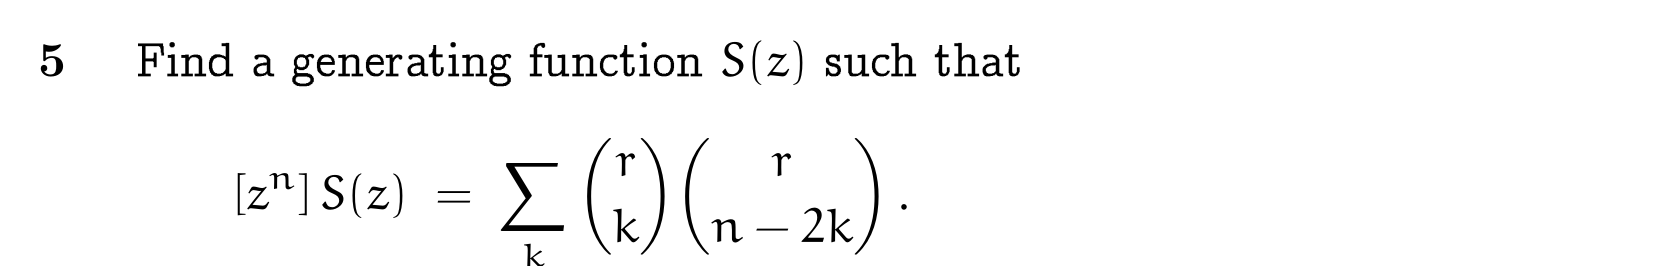
\includegraphics[scale = 0.3]{2023-04-20-11-38-49.png}
\end{figure}
这道题可以通过$[z^n]S(z)$的含义入手。\par 
$[z^n]S(z)$的含义是生成函数$S(z)$中$z^n$项前面的系数.\par
即,
\begin{equation}
    S(z) = \sum_{n}\sum_{k}\binom{r}{k}\binom{r}{n-2k}z^n
\end{equation}
\par 
通过观察所给系数$\binom{r}{k}$和$\binom{r}{n-2k}$,可知,可以通过二项式来凑出系数.\par
这两个二项式是$(1+z)^n$和$(1+z^2)^n$.
所以有
\begin{align}
    (1+z)^r(1+z^2)^r& = \sum_{n}\sum_{n}\binom{r}{k}\binom{r}{n-2k}z^n\\
    &=S(z)
\end{align}
有因为
\begin{equation}
    (1+z)^r(1+z^2)^r = (1+z+z^2+z^3)^r
\end{equation}
所以
\begin{equation}
    S(z) = (1+z+z^2+z^3)^r
\end{equation}

\section*{Basics8}
\begin{figure}[H]

\includegraphics[scale = 0.3]{2023-04-20-12-38-00.png}
\end{figure}
看到题干中待求解式子,第一个想法是卷积。\par 
即,将$\frac{1}{(1-z)^{m+1}}$,$(ln(1-z))^2=(-ln(\frac{1}{1-z}))^2$看成卷积的三个部分。\par 
利用特定生成函数的封闭形式$ln\frac{1}{1-z}=\sum_{n\ge 1}\frac{1}{n}z^n$,以及$\frac{1}{(1-z)^{m+1}}=\sum_{n\ge 0}\binom{m+n}{n}z^n$,
所以,卷积形式为
\begin{equation}
    \frac{(ln(1-z))^2}{(1-z)^{m+1}}=\sum_{i+j+k=n}\frac{1}{i}z^i\frac{1}{j}z^j\binom{m+k}{k}z^k
\end{equation}
\par 
但是这种变换无法求解第9问.
\par 
考虑另外一种思路.
\par 
令$f(x) = (1-z)^{-x-1}$,
利用生成函数进行转换,有
\begin{align}
    f(x)&=\frac{1}{(1-z)^{x+1}}\\
    &=\sum_{n\ge 0}\binom{n+x}{n}z^n\\
    &=\sum_{n\ge 0}\frac{(n+x)(n+x-1)\cdots(x+1)}{n!}z^n
\end{align}
因为需要$ln(1-z)$项,所以需要对$f(x)$求导,有
\begin{align}
    f_{'}(x)&=-(1-z)^{-x-2}ln(1-z)\\
    &=\sum_{n\ge 0}\frac{d}{dx}\frac{(x+n)(x+n-1)\cdots (x+1)}{n!}z^n\\
    &=\sum_{n\ge 0}{(x+n)(x+n-1)\cdots (x+1)}(\frac{1}{x+n} + \cdots + \frac{1}{x+1})\\
    &=\sum_{n\ge 0}\frac{(x+n)(x+n-1)\cdots(x+1)}{n!}z^n(H_{x+n}-H_{x})
\end{align}
同理,再求一次导,有
\begin{align}
    f^{''}(x) &= \sum_{n\ge 0}\frac{(x+n)(x+n-1)\cdots(x+1)}{n!}z^n((H_{x+n}^2-H_{x})^2 - (H^{(2)}_{x+n}-H^{(2)}_{x}))\\
\end{align}
所以,有
\begin{align}
    S(z) &= (1-z)^{-m-1}(ln(1-z))^2\\
    &= f^{''}(x)\\
    &= \sum_{n\ge 0}\frac{(x+n)(x+n-1)\cdots(x+1)}{n!}z^n((H_{x+n}^2-H_{x})^2 - (H^{(2)}_{x+n}-H^{(2)}_{x}))\\
    &=\sum_{n\ge 0}\binom{m+n}{n}z^n((H_{x+n}^2-H_{x})^2 - (H^{(2)}_{x+n}-H^{(2)}_{x}))\\
\end{align}


\section*{Basics9}
\begin{figure}[H]

\includegraphics[scale = 0.3]{2023-04-20-12-38-25.png}
\end{figure}
根据卷积,我们可以得到
\begin{align}
    \frac{(ln(1-z))^2}{(1-z)^2} &= \sum_{n\ge 0}(\sum_{k \ge 0}H_{k}H_{n-k})z^n\\
\end{align}
所以,根据第八题的结论,只需令$m=1$,就有
\begin{align}
    [z^n]S(z) &= \frac{(ln(1-z))^2}{(1-z)^2}\\
    &=\sum_{k \ge 0}H_{k}H_{n-k}\\
    &=\binom{n+1}{n}((H_{n+1} - H_{1})^2 - (H^{(2)}_{n+1}-H^{(2)}_{1}))\\
    &=(n+1)(H_{n}^2 - H^{(2)}_{n})-2n(H_{n} - 1)\\
\end{align}

\end{document}